% The intended deployment around the executed artifact.
%
% The boxes are the same ones as in the executed pipeline, plus the parts of
% the intended deployment that the artifact does not run: multi-observer
% aggregation, the action-dependent state update and the constraint budget.
% Every proposed part is drawn dashed and says so.
%
% (tikz itself is loaded by Definitions/mdpi; the libraries are pulled in here
%  so this file compiles standalone as well as inside the MDPI class.)
\usetikzlibrary{arrows.meta,positioning,calc}

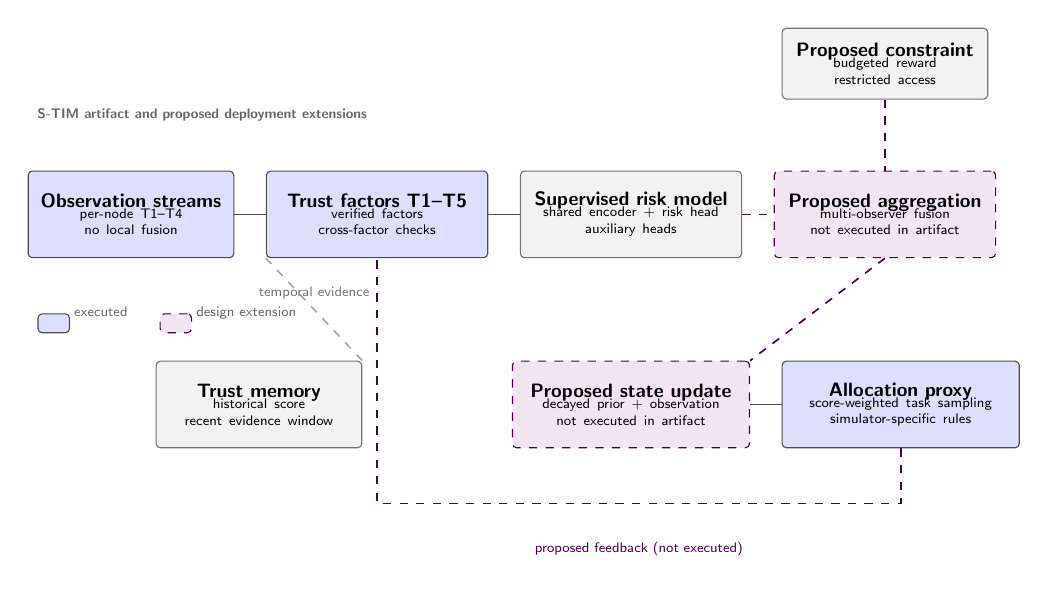
\begin{tikzpicture}[
  font=\sffamily\scriptsize,
  >=Stealth,
  node distance=4mm,
  line/.style={draw=black!70, line width=0.6pt},
  ghostline/.style={draw=black!35, line width=0.6pt, dashed},
  propline/.style={draw=violet!60!black, line width=0.6pt, dashed},
  stage/.style={draw=black!55, fill=black!5, rounded corners=1.5pt, align=center,
                minimum height=11mm, inner xsep=3pt, inner ysep=3pt},
  used/.style={draw=black!70, fill=blue!13, rounded corners=1.5pt, align=center,
               minimum height=11mm, inner xsep=3pt, inner ysep=3pt},
  prop/.style={draw=violet!55!black, fill=violet!10, dashed, rounded corners=1.5pt,
               align=center, minimum height=11mm, inner xsep=3pt, inner ysep=3pt},
  tag/.style={font=\sffamily\tiny, text=black!60, align=center}
]

% ---------------- executed row ----------------
\node[used, text width=24mm] (obs) {
  \textbf{Observation streams}\\[-2pt]{\tiny per-node T1--T4\\[-2pt]no local fusion}};
\node[used, right=of obs, text width=26mm] (fac) {
  \textbf{Trust factors T1--T5}\\[-2pt]{\tiny verified factors\\[-2pt]cross-factor checks}};
\node[stage, right=of fac, text width=26mm] (risk) {
  \textbf{Supervised risk model}\\[-2pt]{\tiny shared encoder + risk head\\[-2pt]auxiliary heads}};
\node[prop, right=of risk, text width=26mm] (agg) {
  \textbf{Proposed aggregation}\\[-2pt]{\tiny multi-observer fusion\\[-2pt]not executed in artifact}};

\draw[line] (obs) -- (fac);
\draw[line] (fac) -- (risk);
\draw[propline] (risk) -- (agg);

\node[stage, above=9mm of agg, text width=24mm, minimum height=9mm] (cons) {
  \textbf{Proposed constraint}\\[-2pt]{\tiny budgeted reward\\[-2pt]restricted access}};
\draw[propline] (cons.south) -- (agg.north);

% ---------------- lower row ----------------
\node[stage, below=13mm of fac, xshift=-15mm, text width=24mm] (mem) {
  \textbf{Trust memory}\\[-2pt]{\tiny historical score\\[-2pt]recent evidence window}};
\node[prop, below=13mm of risk, text width=28mm] (upd) {
  \textbf{Proposed state update}\\[-2pt]{\tiny decayed prior + observation\\[-2pt]not executed in artifact}};
\node[used, right=of upd, text width=28mm] (alloc) {
  \textbf{Allocation proxy}\\[-2pt]{\tiny score-weighted task sampling\\[-2pt]simulator-specific rules}};

\draw[ghostline] (mem.north east) -- node[above, font=\sffamily\tiny, text=black!55] {temporal evidence} (fac.south west);
\draw[propline] (agg.south) -- (upd.north east);
\draw[line] (upd) -- (alloc);

% the closed loop the artifact does not close
\draw[propline] (alloc.south) -- ++(0,-7mm) -| (fac.south);
\coordinate (fb) at ($(fac.south)!0.5!(alloc.south)$);
\node[tag, text=violet!60!black, anchor=south] at ([yshift=-27mm]fb) {proposed feedback (not executed)};

% ---------------- title and legend ----------------
\node[tag, anchor=south west] at ([yshift=5mm]obs.north west) {
  \textbf{S-TIM artifact and proposed deployment extensions}};
\node[tag, anchor=north west] at ([yshift=-5mm]obs.south west) {
  \tikz[baseline=-0.6ex]\node[used, minimum height=2.4mm, minimum width=4mm, inner sep=0pt] {};\hspace{1.5pt}executed
  \hspace{8pt}
  \tikz[baseline=-0.6ex]\node[prop, minimum height=2.4mm, minimum width=4mm, inner sep=0pt] {};\hspace{1.5pt}design extension};

\end{tikzpicture}
